% Created 2023-01-08 dom 16:59
% Intended LaTeX compiler: pdflatex
\documentclass[aspectratio=169, usenames,svgnames,dvipsnames]{beamer}
\usepackage[utf8]{inputenc}
\usepackage[T1]{fontenc}
\usepackage{graphicx}
\usepackage{longtable}
\usepackage{wrapfig}
\usepackage{rotating}
\usepackage[normalem]{ulem}
\usepackage{amsmath}
\usepackage{amssymb}
\usepackage{capt-of}
\usepackage{hyperref}
\usepackage{color}
\usepackage{listings}
\usepackage{mathpazo}
\usepackage{gensymb}
\usepackage{amsmath}
\usepackage{diffcoeff}
\usepackage{steinmetz}
\usepackage{mathtools}
\usepackage{fancyvrb}
\DefineVerbatimEnvironment{verbatim}{Verbatim}{fontsize=\tiny, formatcom = {\color{black!70}}}
\bibliographystyle{plain}
\usepackage{siunitx}
\sisetup{output-decimal-marker={,}}
\DeclareSIUnit{\watthour}{Wh}
\DeclareSIUnit{\wattpeak}{Wp}
\DeclareSIUnit{\watthour}{Wh}
\DeclareSIUnit{\amperehour}{Ah}
\usepackage{steinmetz}
\hypersetup{colorlinks=true, linkcolor=Blue, urlcolor=Blue}
\renewcommand{\thefootnote}{\fnsymbol{footnote}}
\parskip=5pt
\usetheme{Boadilla}
\usecolortheme{rose}
\usefonttheme{serif}
\author{\href{https://oscarperpinan.github.io}{Oscar Perpiñán Lamigueiro}}
\date{}
\title{Control de Calidad de Radiación Solar}
\subtitle{Energía Solar Fotovoltaica}
\institute[UPM]{Universidad Politécnica de Madrid}
\setbeamercolor{alerted text}{fg=blue!50!black} \setbeamerfont{alerted text}{series=\bfseries}
\AtBeginSubsection[]{\begin{frame}[plain]\tableofcontents[currentsubsection,sectionstyle=show/shaded,subsectionstyle=show/shaded/hide]\end{frame}}
\AtBeginSection[]{\begin{frame}[plain]\tableofcontents[currentsection,hideallsubsections]\end{frame}}
\beamertemplatenavigationsymbolsempty
\setbeamertemplate{footline}[frame number]
\setbeamertemplate{itemize items}[triangle]
\setbeamertemplate{enumerate items}[circle]
\setbeamertemplate{section in toc}[circle]
\setbeamertemplate{subsection in toc}[circle]
\hypersetup{
 pdfauthor={\href{https://oscarperpinan.github.io}{Oscar Perpiñán Lamigueiro}},
 pdftitle={Control de Calidad de Radiación Solar},
 pdfkeywords={},
 pdfsubject={},
 pdfcreator={Emacs 28.2 (Org mode 9.6)}, 
 pdflang={Spanish}}
\begin{document}

\maketitle

\section{Estadística}
\label{sec:org9615179}


\begin{frame}[label={sec:org1820aa3}]{Variable aleatoria y proceso estocástico}
\begin{itemize}
\item Una \alert{variable aleatoria} es una función que asigna un único numero
real a cada resultado de un espacio muestral en un experimento.
\item Un \alert{proceso estocástico} es una variable aleatoria que evoluciona a
lo largo del \alert{tiempo} (p.ej. la radiación).
\end{itemize}
\end{frame}


\begin{frame}[label={sec:orgf59fafc}]{Función de densidad de probabilidad}
La función de densidad de probabilidad, \(f(X)\), de una variable
aleatoria \alert{asigna probabilidad} a un suceso:


\[
P(a<X<b)=\int_{a}^{b}f(x)dx
\]


\[
P(X<b)=\int_{-\infty}^{b}f(x)dx\]


\[
P(X>a)=\int_{a}^{\infty}f(x)dx\]
\end{frame}


\begin{frame}[label={sec:org3448d44}]{Función de Densidad de Probabilidad}
\begin{center}
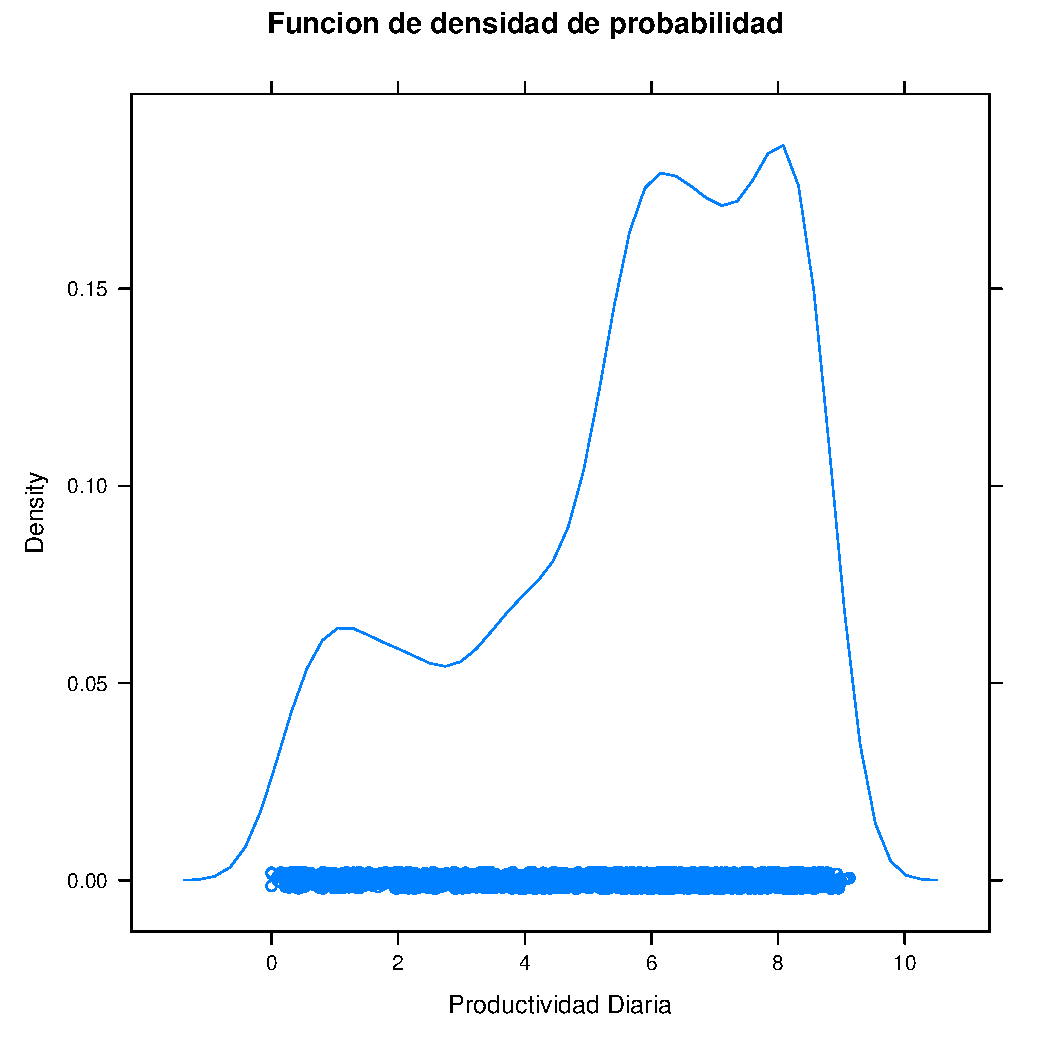
\includegraphics[width=.9\linewidth]{../figs/FuncionDensidadProbabilidad.pdf}
\end{center}
\end{frame}

\begin{frame}[label={sec:orgb075c7e}]{Histograma}
\begin{center}
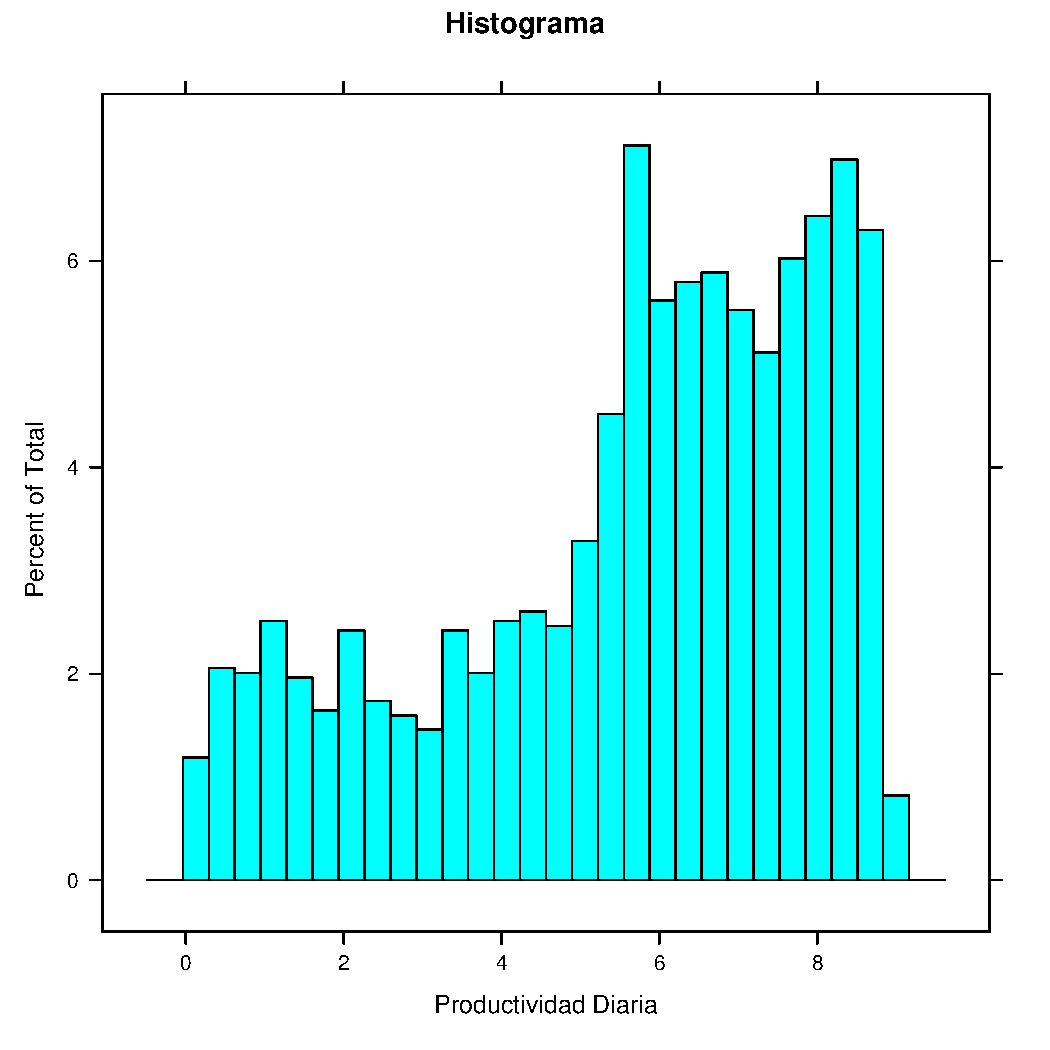
\includegraphics[width=.9\linewidth]{../figs/Histograma.pdf}
\end{center}
\end{frame}



\begin{frame}[label={sec:org9593f34}]{Media, varianza y desviación estándar}
\begin{itemize}
\item La \alert{media} de una variable aleatoria es el \alert{centro de masas} de su función densidad de probabilidad:
\end{itemize}

\[
\mu_{X}=\int_{-\infty}^{\infty}x\cdot f(x)dx
\]

\begin{itemize}
\item La \alert{varianza} de una variable aleatoria es la \alert{media del cuadrado de las desviaciones} respecto a la media:
\end{itemize}

\[
\sigma_{X}^{2}=\int_{-\infty}^{\infty}(x-\mu_{X})^{2}\cdot f(x)dx
\]

\begin{itemize}
\item La \alert{desviación estándar} es la raiz cuadrada de la varianza: \(\sigma_{X}=\sqrt{\sigma_{X}^2}\)
\end{itemize}
\end{frame}



\begin{frame}[label={sec:org4a220fe}]{Combinación lineal de variables aleatorias}
\begin{itemize}
\item La \alert{media de la suma} de varias variables aleatorias \alert{independientes} es
la suma de las medias:
\end{itemize}
\[
\mu_{X_{1}+...+X_{n}}=\mu_{X_{1}}+...+\mu_{X_{n}}
\]

\begin{itemize}
\item La \alert{varianza de la \emph{suma o resta}} de varias variables aleatorias
\alert{independientes} es la \alert{suma} de las varianzas:
\end{itemize}

\[
\sigma_{X_{1}\pm...\pm X_{n}}^{2}=\sigma_{X_{1}}^{2}+...+\sigma_{X_{n}}^{2}
\]
\end{frame}



\begin{frame}[label={sec:orgd4a7f0a}]{Media y varianza de la media muestral}
\begin{itemize}
\item Una \alert{muestra de una población} es un conjunto de variables
aleatorias independientes (\(X_{1}...X_{n}\)).

\item Si se toma una muestra de una población cuya media es \(\mu\) y su
varianza es \(\sigma^{2}\), entonces la media de la muestra es otra
variable aleatoria (que es una suma de variables aleatorias)
\end{itemize}

\[
\overline{X}=\frac{1}{n}\sum_{n}X_{i}
\]
\end{frame}



\begin{frame}[label={sec:org5491931}]{Media y varianza de la media muestral}
\begin{itemize}
\item Por tanto, la \alert{media de la media muestral} es la media de población:
\end{itemize}
\[
\overline{X}=\frac{1}{n}\sum_{n}X_{i} = \mu
\]

\begin{itemize}
\item La \alert{varianza de la media muestral} es la suma de las varianzas:
\end{itemize}

\[
\sigma_{\overline{X}}^{2}=\sigma_{\frac{1}{n}X_{1}}^{2}+...+\sigma_{\frac{1}{n}X_{n}}^{2}=\frac{\sigma^2}{N}
\]

\begin{block}{}
Por tanto, una forma de \alert{reducir la incertidumbre} es realizar la
\alert{medida en repetidas ocasiones}.
\end{block}
\end{frame}



\begin{frame}[label={sec:org60c7299}]{Mediana y cuartiles}
\begin{itemize}
\item La \alert{mediana} divide el conjunto de valores de la variable en \alert{dos
mitades} iguales (divide el area encerrada por la función densidad
de probabilidad en dos partes iguales).
\item Los \alert{cuartiles} dividen este area en \alert{cuatro} partes iguales.
\item El area encerrada entre cada par de cuartiles es igual al 25$\backslash$% del total.
\item La \alert{mediana} es el \alert{segundo cuartil}.
\item La \alert{distancia intercuartil} (definida entre los cuartiles 1 y 3) es
una \alert{medida de la dispersión} de la variable.
\end{itemize}
\end{frame}


\section{Gráficos}
\label{sec:orgaecbcce}


\begin{frame}[label={sec:orga36dcca}]{Función de Densidad de Probabilidad}
\begin{center}
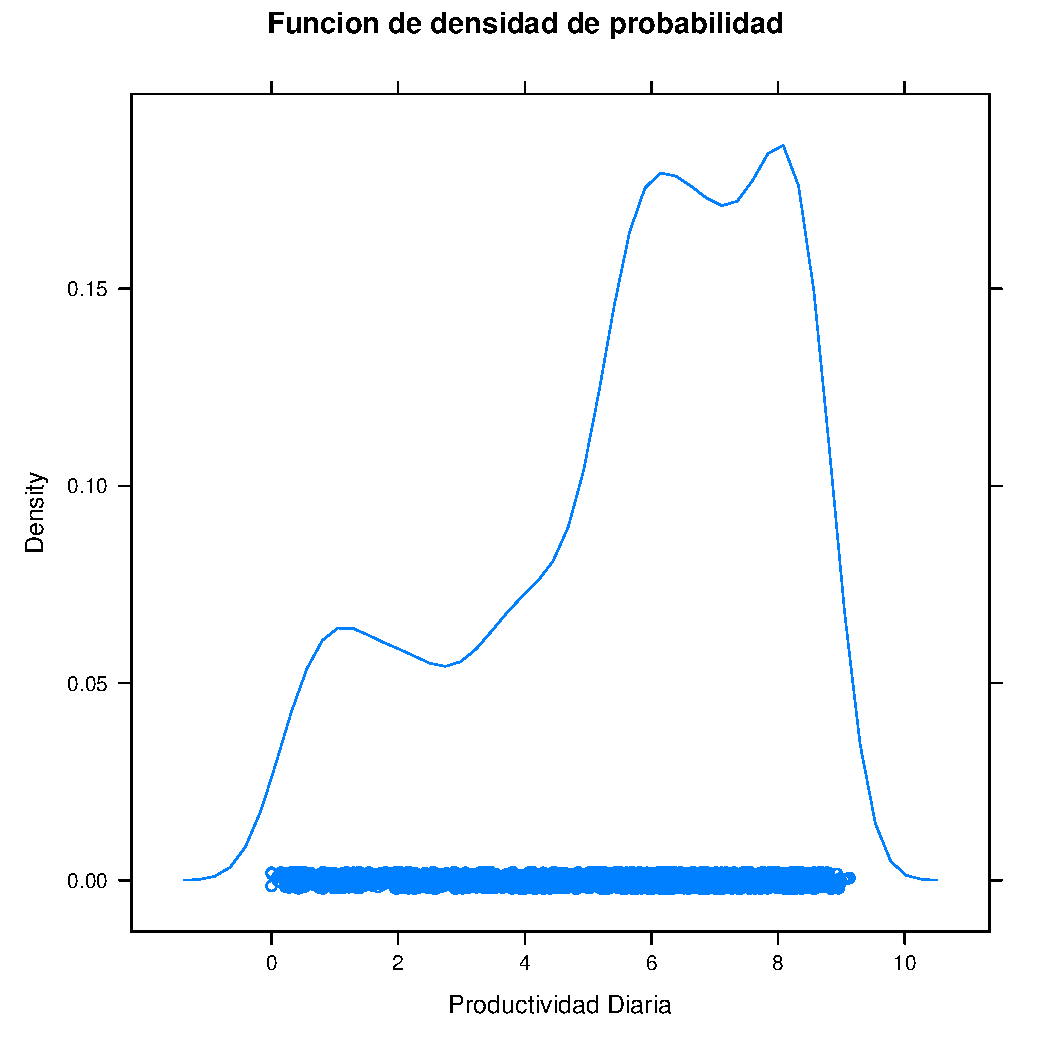
\includegraphics[width=.9\linewidth]{../figs/FuncionDensidadProbabilidad.pdf}
\end{center}
\end{frame}

\begin{frame}[label={sec:orge16c279}]{Histograma}
\begin{center}
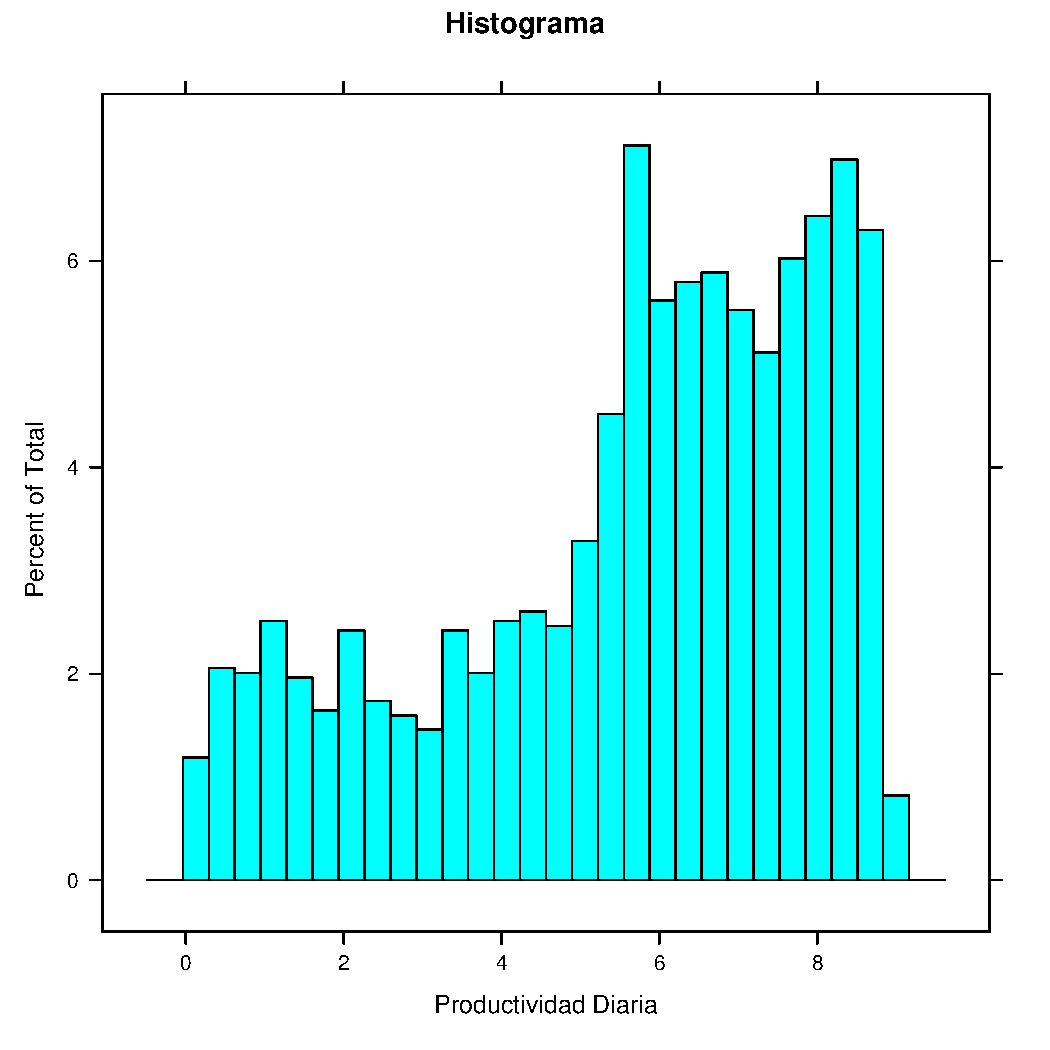
\includegraphics[width=.9\linewidth]{../figs/Histograma.pdf}
\end{center}
\end{frame}


\begin{frame}[label={sec:org2de4989}]{Gráficos boxplot}
\begin{center}
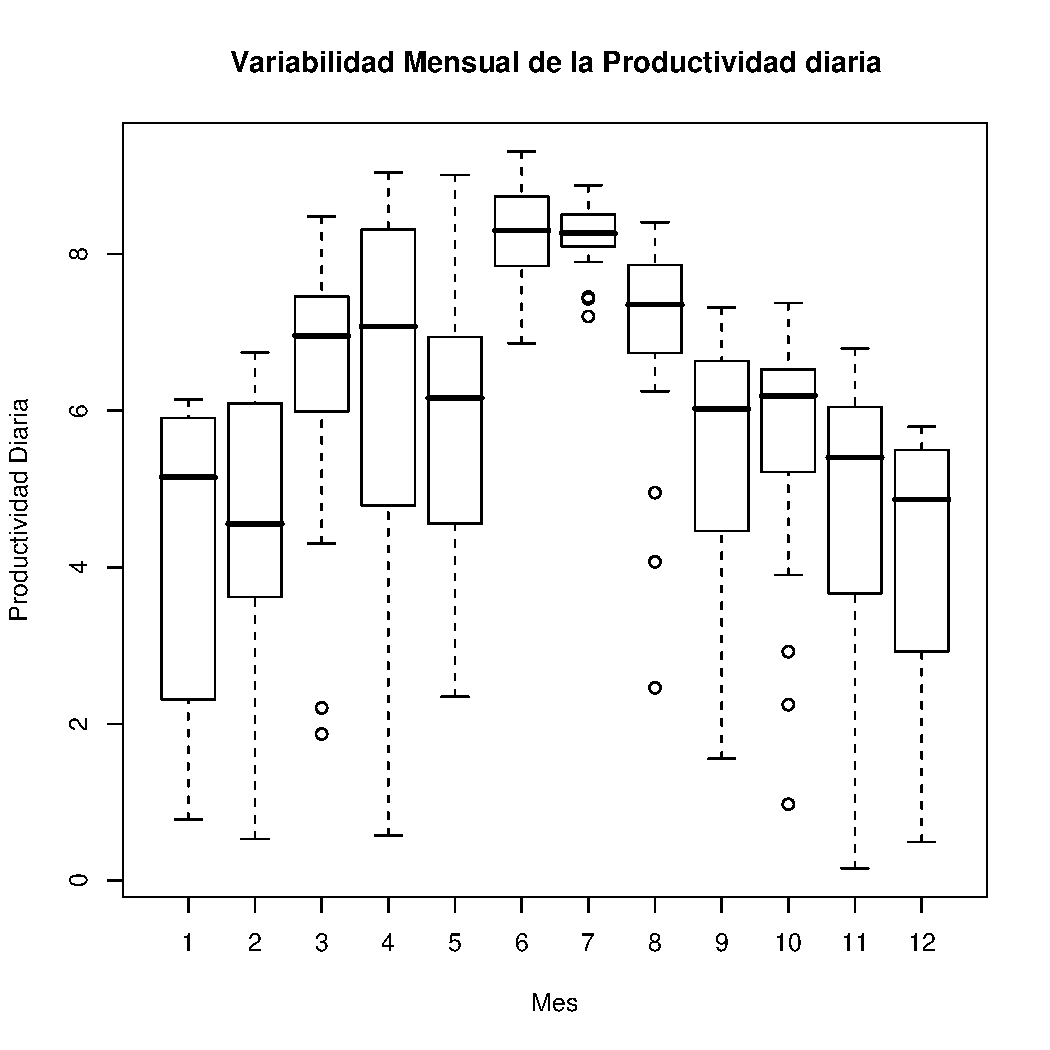
\includegraphics[width=.9\linewidth]{../figs/GraficoBoxplot.pdf}
\end{center}
\end{frame}


\begin{frame}[label={sec:orge02437b}]{Gráficos de dispersión}
\begin{center}
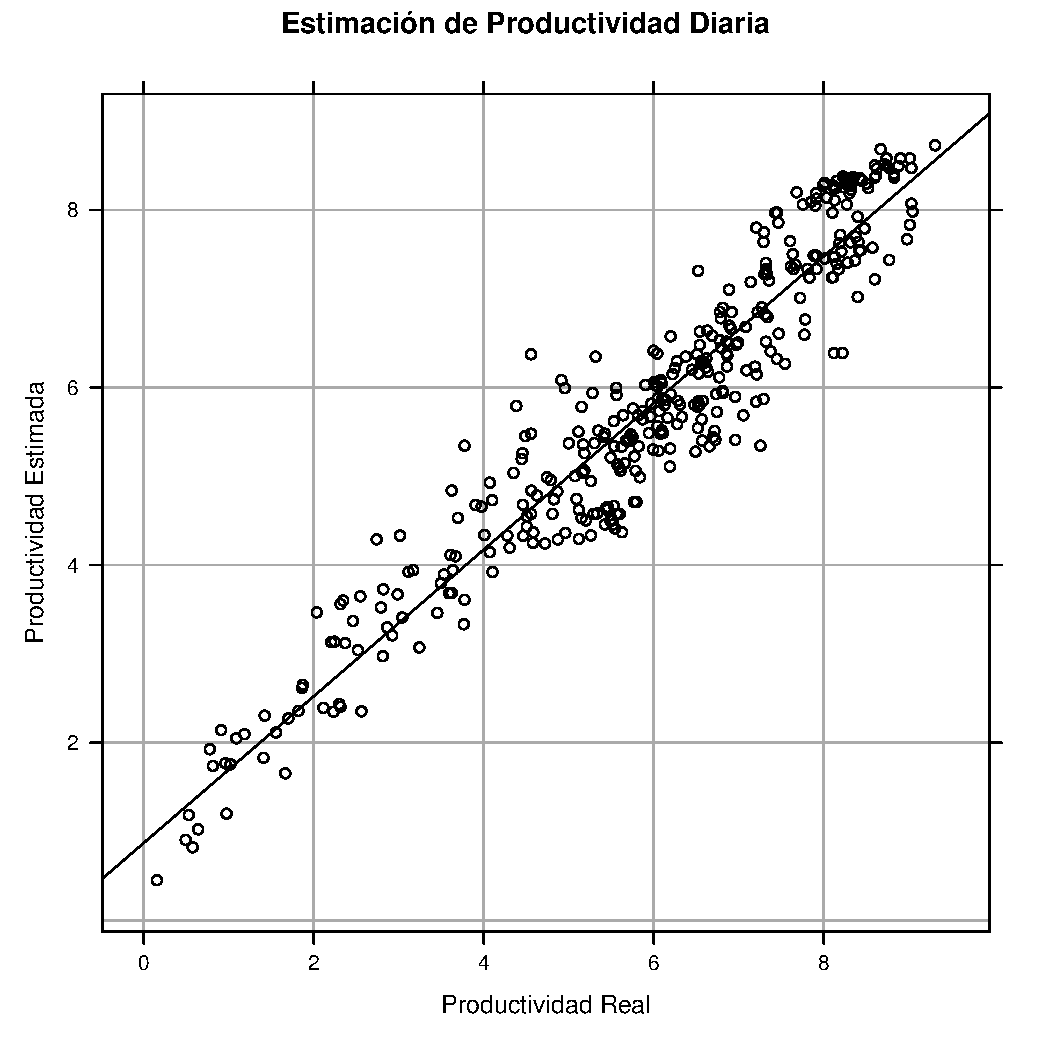
\includegraphics[width=.9\linewidth]{../figs/GraficoDispersion.pdf}
\end{center}
\end{frame}


\begin{frame}[label={sec:org0ec8ed9}]{Matrices de gráficos de dispersión}
\begin{center}
\includegraphics[height=0.9\textheight]{../figs/Splom.png}
\end{center}
\end{frame}

\section{Control de Calidad de Medidas}
\label{sec:orga4a0710}

\begin{frame}[label={sec:org31878d4}]{Introducción}
\begin{block}{Las medidas recogidas por estaciones meteorológicas se deben filtrar para eliminar datos erroneos.}
\begin{itemize}
\item Límites Físicos
\item Tests de persistencia
\item Tests de rampas (irradiancia)
\item Tests de envolvente (medida de varias componentes)
\item Coherencia espacial
\item Coherencia estadística
\end{itemize}
\end{block}
\end{frame}



\begin{frame}[label={sec:org2d67bf8}]{Límites físicos}
\begin{block}{Irradiación Diaria}
\begin{itemize}
\item La radiación global en el plano horizontal debe ser inferior a la extraterrestre (\(K_t \leq 1\))
\end{itemize}
\[
G_d(0) \leq B_od(0)
\]

\begin{itemize}
\item El índice de claridad debe ser superior a 0.03
\end{itemize}
\[
K_t = \frac{G_d(0)}{B_{od}(0)} \geq 0.03
\]

\begin{itemize}
\item La radiación global en el plano horizontal debe ser inferior a la de un modelo de cielo claro
\end{itemize}

\nocite{Younes.Claywell.ea2005, Estevez.Gavilan.ea2011, Geiger.Diabate.ea2002}
\end{block}
\end{frame}

\begin{frame}[label={sec:org9583982}]{Límites físicos}
\begin{block}{Irradiancia (intradiaria)}
\begin{itemize}
\item El índice de claridad debe ser inferior a 1 cuando la altura solar es suficiente:
\end{itemize}
\[
k_t < 1  \text{ si } \gamma_s > 2\degree 
\]
\begin{itemize}
\item Límites inferiores para cielos cubiertos (baja transparencia atmosférica)
\end{itemize}
\[
k_t \geq 10^{-4} \cdot (\gamma_s - 10\degree)  \text{ si } \gamma_s > 10\degree
\]

\[
G \geq 0  \text{ si } \gamma_s \leq 10\degree
\]

\nocite{Journee.Bertrand2011}
\end{block}
\end{frame}

\begin{frame}[label={sec:org833448a}]{Tests de persistencia}
\begin{block}{Variabilidad de irradiancia}
\begin{itemize}
\item La media y la desviación estándar se calculan con todas las muestras de un día completo.
\end{itemize}
\[
\frac{1}{8} \overline{k_t} \leq \sigma_{k_t} \leq 0.35
\]
\end{block}
\end{frame}

\begin{frame}[label={sec:org64f1b2d}]{Tests de rampas}
\begin{block}{Límites a las variaciones de la irradiancia entre instantes sucesivos}
\[
\left| k_t(t) - k_t(t-1)\right| < 0.75 \text{ si } \gamma_s(t) > 2\degree
\]
\end{block}
\end{frame}


\begin{frame}[label={sec:orgb7883e0}]{Tests de envolvente}
\begin{itemize}
\item Sólo para estaciones con medida simultánea de global y directa/difusa.
\end{itemize}

\begin{center}
\includegraphics[width=.9\linewidth]{../figs/ConsistencyTest.png}
\end{center}

\nocite{Younes.Claywell.ea2005}
\end{frame}

\begin{frame}[label={sec:org13dbe26}]{Coherencia espacial}
\begin{itemize}
\item Las medidas de una estación se pueden comparar con las recogidas por estaciones cercanas.
\item Esta comprobación debe realizarse con \alert{datos agregados} (diarios) (la variabilidad espacial intradiaria puede ser alta)
\item Esta comprobación debe realizarse con estaciones que tienen \alert{clima y geografía similar}.
\end{itemize}

\nocite{Journee.Bertrand2011}
\end{frame}

\begin{frame}[label={sec:orgd1c9fa9}]{Coherencia espacial}
\begin{block}{Pasos}
\begin{itemize}
\item Estimamos la irradiación en el lugar, \(x_0\), con la interpolación espacial de las estaciones cercanas, \(x_i\).
\begin{itemize}
\item Los pesos \(w_i\) son una función inversa de la distancia (IDW).
\end{itemize}
\end{itemize}
\[
\widehat{G}_d(x_0) = \frac{\sum_{i=1}^N w_i G_{d}(x_i)}{\sum_{i=1}^N w_i} 
\]
\begin{itemize}
\item Comparamos la irradiación estimada, \(\widehat{G}_d(x_0)\), con la medida en la estación, \(G_d(x_0)\).
\end{itemize}
\[
\left| \widehat{G}_d(x_0) - G_d(x_0) \right|
\]
\begin{itemize}
\item La diferencia absoluta debe estar por debajo de un límite (p.ej. 50\%)
\end{itemize}
\end{block}
\end{frame}



\begin{frame}[label={sec:org12df237}]{Coherencia estadística}
\begin{block}{Una medida puede ser etiquetada como \emph{outlier} si es poco probable que pertenezca a la misma distribución que el conjunto.}
\end{block}
\begin{block}{\alert{Método de Chauvenet}}
Una medida es un \emph{outlier} si la probabilidad de obtener su desviación
respecto de la media es inferior al inverso de 2 veces el número de
elementos en el conjunto.

\begin{center}
\includegraphics[width=.9\linewidth]{../figs/chauvenet.png}
\end{center}
\end{block}
\end{frame}

\begin{frame}[label={sec:org46c0645}]{Método de Chauvenet}
\begin{itemize}
\item Sean \(G_d(x_i)\) las medidas de radiación diaria del conjunto formado por N estaciones.
\end{itemize}

\pause

\begin{itemize}
\item Se calcula la media, \(\overline{G}_d\), la desviación estándar, \(\sigma_{G_d}\).
\end{itemize}

\pause

\begin{itemize}
\item Se calcula la distancia estadística de cada estación al conjunto:
\end{itemize}
\[
d_i = \frac{G_d(x_i) - \overline{G}_d}{\sigma_{G_d}}
\]

\pause

\begin{itemize}
\item En una distribución gaussiana se calcula la distancia estadística
equivalente a la probabilidad límite, \(1/2N\), teniendo en cuenta
las dos colas.
\begin{itemize}
\item Por ejemplo, para un conjunto de 10 estaciones cada cola es
\(1/40 = 0.025\), el límite es \(\left| d_{max} \right| = 1.96\).
\end{itemize}
\end{itemize}
\pause

\begin{itemize}
\item Aquellas observaciones que superan la distancia son marcadas como outliers.
\end{itemize}

\nocite{Perpinan2009}
\end{frame}

\begin{frame}[label={sec:org93a770f}]{Método de Chauvenet}
\[
d_i = \frac{G_d(x_i) - \overline{G}_d}{\sigma_{G_d}}
\]

\[
\left| d_i \right| > \left| d_{max} \right|
\]

\begin{center}
\begin{center}
\includegraphics[width=.9\linewidth]{../figs/chauvenet.png}
\end{center}
\end{center}

\begin{block}{Método de Pierce: más robusto y flexible \nocite{Ross2003}}
\end{block}
\end{frame}

\section{Control de Calidad de Modelos}
\label{sec:org31d94ba}

\begin{frame}[label={sec:orgf34cc7a}]{Desviación entre modelo y observación}
\begin{itemize}
\item Sea \(O\) el conjunto de observaciones (medidas) de una variable aleatoria.
\end{itemize}

\[
\mathbf{O} = \left\{ o_1 \dots o_n \right\}
\]
\begin{itemize}
\item Sea \(M\) el conjunto de resultados de un modelo que aproxima el comportamiento de la variable medida.
\end{itemize}

\[
\mathbf{M} = \left\{ m_1 \dots m_n  \right\}
\]

\begin{itemize}
\item La desviación entre modelo y observación es:
\end{itemize}

\[
\mathbf{D} = \mathbf{M} - \mathbf{O} =  \left\{ (m_1 - o_1) \dots (m_n - o_n)  \right\} = \left\{ d_1 \dots d_n  \right\}
\]
\end{frame}

\begin{frame}[label={sec:org8ed2567}]{Estimadores frecuentes: MBD y RMSD}
\begin{itemize}
\item Mean Bias Difference (MBD), diferencia media (indica si el modelo sobreestima o subestima):
\end{itemize}
\[
MBE = \overline{\mathbf{D}} = \overline{\mathbf{M}} - \overline{\mathbf{O}} = \frac{1}{n} \sum_{i=1}^n (m_i - o_i)
\]
\pause
\begin{itemize}
\item Root Mean Square Error (RMSD), diferencia cuadrático media:
\end{itemize}
\[
RMSD = \left(\frac{1}{n} \sum_{i=1}^n d_i^2 \right)^{1/2} =  \left( \frac{1}{n} \sum_{i=1}^n (m_i - o_i)^2  \right)^{1/2}
\]
\end{frame}

\begin{frame}[label={sec:org12d5274}]{Estimadores frecuentes: MBE y RMSD}
\begin{itemize}
\item Varianza de la diferencia (unbiased RMSD):
\end{itemize}
\[
\sigma^2_{\mathbf{D}} = \frac{1}{n} \sum_{i=1}^n (d_i - \overline{\mathbf{D}})^2
\]
\pause

\begin{itemize}
\item El RMSD agrega información del promedio y la varianza de la
diferencia:
\end{itemize}
\[
RMSD^2= \sigma^2_{\mathbf{D}} + \overline{\mathbf{D}}^2
\]
\end{frame}

\begin{frame}[label={sec:org8b35dea}]{Otros estimadores: MAD}
\begin{itemize}
\item Mean Absolute Deviation (MAD):
\end{itemize}

\[
MAD = \frac{1}{n} \sum_{i=1}^n \left|d_i\right| =  \frac{1}{n} \sum_{i=1}^n \left|m_i - o_i\right|
\]
\begin{itemize}
\item El RMSD no es robusto (un error puntual puede distorsionar el estimador) y depende del número de muestras:
\end{itemize}
\[
MAD \leq RMSD \leq n^{1/2} MAD
\]

\nocite{Willmott.Matsuura.ea2009, Willmott.Matsuura2005a}
\end{frame}

\begin{frame}[label={sec:org5ada187}]{Otros estimadores: t y d}
\begin{itemize}
\item t de Student (valores pequeños indican buen comportamiento del modelo)
\begin{itemize}
\item Permite añadir intervalos de confianza a las diferencias entre
modelo y observación
\end{itemize}
\end{itemize}

\[
t = \left ( \frac{(n-1) MBD^2}{RMSD^2 - MBD^2} \right)^{1/2}
\]

\nocite{Stone1993}

\pause 

\begin{itemize}
\item \(d_1\): Índice de concordancia de Willmott.
\begin{itemize}
\item Limitado entre 0 (ausencia de concordancia) y 1 (concordancia total).
\item Robusto frente a \emph{outliers}.
\end{itemize}
\end{itemize}
\[
d_1 = 1 - \frac{\sum_{i=1}^n \left| m_i - o_i \right|}{\sum_{i=1}^n \left(
  \left| m_i - \overline{\mathbf{O}}\right| + \left| o_i -
    \overline{\mathbf{O}} \right| \right)}
\]

\nocite{Willmott.Robeson.ea2012}
\end{frame}

\begin{frame}[label={sec:org4718b92}]{Correlación}
El coeficiente de correlación entre dos conjuntos de datos es una
medida numérica de la relación \alert{lineal} entre los dos conjuntos (si la
relación no es lineal, este coeficiente no sirve):

\[
r = \frac{1}{n-1} \cdot \sum_{i=1}^{n} \left( \frac{o_{i}-\overline{\mathbf{O}}}{\sigma_{\mathbf{O}}}\right) \cdot \left(\frac{m_{i}-\overline{\mathbf{M}}}{\sigma_{\mathbf{M}}}\right)
\]
\end{frame}

\begin{frame}[label={sec:org066f671}]{Diagramas de Taylor}
\begin{itemize}
\item Desarrollando \(\sigma^2_{\mathbf{D}}\) y teniendo en cuenta la definición de \(r\):
\end{itemize}

  \[
  \sigma^2_{\mathbf{D}} = \sigma^2_{\mathbf{O}}  + \sigma^2_{\mathbf{M}}
- 2 \cdot \sigma_{\mathbf{O}} \cdot \sigma_{\mathbf{M}} \cdot r
  \]
\begin{itemize}
\item Esta relación es semejante a la ley de los cosenos (\(c\), \(a\), \(b\) son lados de un triángulo y \(\phi\) es el ángulo opuesto al lado \(c\)):
\end{itemize}

\[
c^2 = a^2 + b^2 - 2 \cdot a \cdot b \cos\phi
\]
\nocite{Taylor2000}
\end{frame}

\begin{frame}[label={sec:orga2e42b5}]{Diagramas de Taylor}
\[
\sigma^2_{\mathbf{D}} = \sigma^2_{\mathbf{O}}  + \sigma^2_{\mathbf{M}}
- 2 \cdot \sigma_{\mathbf{O}} \cdot \sigma_{\mathbf{M}} \cdot r 
\]

\begin{center}
\begin{center}
\includegraphics[width=.9\linewidth]{../figs/cosenosDiagramaTaylor.png}
\end{center}
\end{center}
\end{frame}

\begin{frame}[label={sec:org156f7c8}]{Diagramas de Taylor}
\begin{itemize}
\item \(\sigma^2_{\mathbf{D}}\): Distancia al origen
\item \(\sigma^2_{\mathbf{O}}\): Eje horizontal
\item \(\sigma^2_{\mathbf{M}}\): Eje vertical
\item \(r\): acimut
\end{itemize}
\begin{center}
\begin{center}
\includegraphics[height=0.6\textheight]{../figs/TaylorDiagrama.png}
\end{center}
\end{center}
\end{frame}


\begin{frame}[label={sec:org8ae2df4}]{Target Diagram}
\begin{itemize}
\item Emplea la relación entre \(RMSD\), \(\sigma^2_{\mathbf{D}}\), y \(\overline{\mathbf{D}}\), normalizadas con \(\sigma_{\mathbf{O}}\):
\end{itemize}
\[
RMSD' = RMSD / \sigma_{\mathbf{O}}
\]

\[
  \sigma'_{\mathbf{D}} = \sigma_{\mathbf{D}} / \sigma_{\mathbf{O}} 
\]

\[
\overline{\mathbf{D}}' = \overline{\mathbf{D}} / \sigma_{\mathbf{O}}
\]

\[
RMSD'^2= \sigma'^2_{\mathbf{D}} + \overline{\mathbf{D}}'^2
\]

\[
sign_{\sigma} =  sign(\sigma_{\mathbf{M}} - \sigma_{\mathbf{O}} )
\]

\begin{itemize}
\item Incorporan el signo de la diferencia entre desviaciones estándar de modelo y observación:
\end{itemize}

\nocite{Jolliff.Kindle.ea2009}
\end{frame}

\begin{frame}[label={sec:orgbe630e4}]{Target Diagram}
\begin{itemize}
\item \(\sigma'_{\mathbf{D}}\) (con signo): Eje horizontal
\item \(\overline{\mathbf{D}}'\): Eje vertical
\item \(RMSD'^2\): Distancia al origen
\end{itemize}

\begin{center}
\begin{center}
\includegraphics[height=0.7\textheight]{../figs/TargetDiagram.pdf}
\end{center}
\end{center}
\end{frame}
\end{document}